\chapter*{\chapterstyle{IX --- Introduction}}
\addcontentsline{toc}{section}{Introduction} 
Soit \(n, p\) des entiers et \(F\) une fonction \textbf{continue} sur \(\Omega \subseteq \R \times (\R^{p})^n\), alors on appelle \textbf{équation différentielle ordinaire} d'ordre \(n\) tout équation de la forme:
\[
   F(t, y(t), \ldots, y^{(n)}(t)) = 0
\]
Où \(y\) est une fonction d'un intervalle \( I \) dans \(\R^p\) à déterminer. Par exemple, on pose:
\[
   \begin{cases}
      F_1(t, y, y') = y'(t) - y(t)\\
      F_2(t, y, y') = cos(t)y'(t) - y^2(t)\\
      F_3(t, y, y') = 3 + arctan(t) + y'(t) - e^xy(t)\\ 
      F_4(t, y, y', y'') = t^2 + 3y(t)y'(t) + cos(y''(t))
   \end{cases} \implies
   \begin{cases}
      E_1 : y'(t) - y(t) = 0 \\
      E_2 : cos(t)y'(t) - y^2(t) = 0 \\
      E_3 : 3 + arctan(t) + y'(t) - e^xy(t) = 0 \\
      E_4 : t^2 + 3y(t)y'(t) + cos(y''(t)) = 0
   \end{cases}
\]
On peut aussi remarque que cette définition permet à \(y\) d'être à valeurs vectorielles et dans ce cas on obtient alors un \textbf{système différentiel}, par exemple pour \(E = \R^2\) et \(F_1\), on obtient:
\[
   E : \begin{cases}
      y'_1(t) = y_1(t)\\
      y'_2(t) = y_2(t)
   \end{cases}
\]
\subsection*{\subsecstyle{Forme résolue{:}}}
Dans des cas trés précieux, on peut isoler la plus grand dérivée, et on dira alors que l'équation différentielle est \textbf{sous forme résolue} si et seulement si il existe une fonction \(F\) continue sur \(\R \times (\R^p)^{n}\) telle que:
\[
   y^{(n)}(t) = F(t, y(t), \ldots, y^{(n-1)}(t))
\]
On ne s'intéressera dans ce cours qu'à ce cas particulier pour simplifier la compréhension, sauf cas simples où l'on peut se ramener à une forme réduite. Par la suite on appelera \textbf{équation associée à \( F \)} d'ordre \( n \) une équation de la forme ci-dessus.
\subsection*{\subsecstyle{Solution d'une équation différentielle{:}}}
On dira que \((I, y)\) est une \textbf{solution} de l'équation différentiellé d'ordre \( n \) associée à \( F \) si et seulement si \( I \) est un intervalle, \(y \in \mathcal{C}^n(I, \R^p)\) et que:
\[ 
   \forall t \in I \; ; \; (t, y(t), \ldots, y^{(n-1)}(t)) \in \Omega \; \text{ et } \; y^{(n)}(t) = F(t, y(t), \ldots, y^{(n-1)}(t))
\]
On remarque alors que le domaine de définition d'une même fonction solution peut changer et on peut alors définir une notion de solution \textbf{maximale et globale} par:
\begin{itemize}
   \item Une solution est \textbf{maximale} si et seulement si elle ne peut pas être prolongée en une autre solution définie sur une intervalle.
   \item Une solution est \textbf{globale} si et seulement \( \Omega \) est de la forme \(I \times (\R^p)^{n}\) et que \( y \) est une solution définie sur \( I \).
\end{itemize}
\subsection*{\subsecstyle{Réduction de l'ordre{:}}}
On se donne une équations différentielle résolue d'ordre \(n\), alors on pose:
\[
   Y(t) := \begin{pmatrix}
      y(t)\\
      y'(t)\\
      \vdots\\
      y^{(n-1)}(t)
   \end{pmatrix} \quad \quad \quad \quad\quad
   \mathbb{F}(t, Y(t)) := \begin{pmatrix}
      y'(t)\\
      y''(t)\\
      \vdots\\
      F(t, Y(t))
   \end{pmatrix}
\]
Alors on a directement que:
\[
   y^{(n)}(x) = F(x, y(x), \ldots, y^{(n-1)}(x)) \Longleftrightarrow Y'(x) = \mathbb{F}(x, Y(x))
\]
\begin{center}
   \textit{Fondamentalement, comprendre les EDO à l'ordre 1 c'est comprendre toutes les EDO.}
\end{center}
\subsection*{\subsecstyle{Problème de Cauchy{:}}}
Etant donné une équation d'ordre 1, et \( (t_0, y_0) \in \Omega \), on appele \textbf{problème de Cauchy} associée à l'équation \( (E) \) le problème suivant:
\[ 
   P: \begin{cases}
      y' = f(t, y)\\
      y(t_0) = y_0
   \end{cases} 
\]
Une question fondamentale de la théorie des equations differentielles ordinaires consiste à savoir sous quelles hypothèses sur \(  f \)tout problème de Cauchy associé à une équation admet une solution et les propriété de celles ci.
\subsection*{\subsecstyle{Raccordement de solutions{:}}}
Si on obtient deux solutions \( ( \ioo{a}{b}, y_1), (\ioo{b}{c}, y_2) \), alors on peut s'intéresser à raccorder ces deux solutions en une unique solution sur \( \ioo{a}{c} \). C'est en fait possible sous la condition suivante:
\[ 
   \lim_{x \rightarrow b} y_1(b) = \lim_{x \rightarrow b} y_2(b)
\]
\subsection*{\subsecstyle{Expression intégrale des solutions{:}}}
Considérons l'équation du premier ordre \((E)\) et le problème de Cauchy associé au couple \( (t_0, y_0) \), alors \( y \) est solution du problème de Cauchy ssi:
\[ 
   \forall t \in I \; ; \; y(t) = y_0 + \int_{t_0}^t f(s, y(s))ds 
\]
En réinterprétant cette équation et en définissant l'opérateur suivant:
\[ 
   \Phi : y \in \mathcal{C}^0(I, \R^p) \longmapsto (t \mapsto y_0 + \int_{t_0}^t f(s, y(s))ds) \in \mathcal{C}^0(I, \R^p)
\]
Alors une solution est exactement un \textbf{point fixe} de cet opérateur.

\subsection*{\subsecstyle{Equations à paramêtres{:}}}
On peut aussi pour tout paramêtre \( \lambda \in \Lambda \), où \( \Lambda \) est un espace vectoriel de dimension finie, définir une \textbf{équation différentielle à paramètre}, de la forme:
\[ 
   (E_\lambda) : y'(t) = f_\lambda(t, y(t)) 
\]
Résoudre une telle équation revient alors à résoudre une famille d'équations différentielles.
\chapter*{\chapterstyle{IX --- Théorie linéaire}}
\addcontentsline{toc}{section}{Théorie linéaire} 
On appele donc une équation différentielle linéaire une équation différentielle de la forme suivante:
\[ 
   y'(t) = A(t)y(t) + B(t) 
\]
Où \(A \in \mathcal{C}^0(I, \mathcal{M}_p( \K))\) et \(B \in \mathcal{C}^0(I, \mathcal{M}_{p, 1}( \K))\). Ce type d'équation trés spécifique permet d'utiliser la théorie de l'algèbre linéaire pour en trouver des solutions et/ou étudier leurs solutions.
\subsection*{\subsecstyle{Théorème de Cauchy-Lipschitz linéaire{:}}}
Alors gràce au théorème de Banach-Picard et à l'opérateur intégral défini plus haut, on peut montrer le résultat fondamental suivant, si on considère le problème de Cauchy linéaire suivant:
\[ 
   P: \begin{cases}
      y' = A(t)y(t) + B(t)\\
      y(t_0) = y_0
   \end{cases} 
\]
Alors on peut montrer le théorème dit de \textbf{Cauchy-Lipschitz linéaire}:
\begin{center}
   Ce problème admet une \textbf{unique solution} et elle est \textbf{globale}.
\end{center}
\subsection*{\subsecstyle{Exponentielle matricielle{:}}}
Dans le cas linéaire, on peut généraliser la résolution de l'équation élémentaire \( y'(t) = a(t)y(t) \) en étandant le domaine de définition de la fonction exponentielle, en effet pour tout matrice \( A \in \mathcal{M}_n(\K) \), on définit:
\[ 
   e^A = \sum_{n \in \N} \frac{A^n}{n!} 
\]
En effet, on munit \( \mathcal{M}_n(\K) \) d'une norme matricielle, et on peut alors montrer que cette série converge normalement, donc converge car \( \mathcal{M}_n(\K) \) est complet. On peut alors montrer les propriétés suivantes:
\begin{itemize}
   \item On a \( e^0 = 1\).
   \item On a \( e^A \) est inversible d'inverse \( e^{-A} \).
   \item On a \( e^{A+B} = e^Ae^B \) si \( A \) et \( B \) commutent.
\end{itemize}
Si on considère plus généralement une fonction matricielle \( A(t) \in \mathcal{C}^1\), et que \( A(t), A'(t) \) \textbf{commutent} alors on peut montrer que \(t \mapsto e^{A(t)} \) est dérivable de dérivée \( A'(t)e^{A(t)} \).
\subsection*{\subsecstyle{Structure de l'ensemble des solutions{:}}}
On se pose alors la question suivante:
\begin{center}
   \textit{Dans le cas linéaire, est ce que l'ensemble de solutions est muni d'un structure particulière ?}
\end{center}
On peut en effet répondre par l'affirmative, mais définissons tout d'abord quelques notions de vocabulaire, on appelle \textbf{équation homogène} associée à \( (E) \) l'équation différentielle suivante:
\[ 
   (E_H): y'(t) = A(t)y(t) 
\]
Alors on peut montrer que l'ensemble des solutions de cette équation est un \textbf{sous-espace vectoriel} de l'espace \( \mathcal{C}^1(I, \K^n) \), en particulier, la fonction qui a toute solution \( y \) associe son évaluation en \( t_0 \in I \) est un isomorphisme. En outre on peut alors montrer le résultat suivant:
\begin{center}
   \textbf{L'ensemble des solutions de \( E \) est un sous-espace affine de direction \( S_H \).}
\end{center}
Alors en particulier il suffit d'avoir la donnée de \( S_H \) ainsi qu'une solution de \( E \) pour obtenir la solution générale qui sera de la forme:
\[ 
   y_G(t) = y_H(t) + y_P(t) 
\]
Où \( y_H(t) \) est une solution homogène quelconque et \( y_P(t) \) une solution particulière de \( E \). Les sections suivantes visent alors à expliquer comment trouver ces solutions.
\subsection*{\subsecstyle{Système fondamental et wronskien{:}}}
On définit les notions suivantes:
\begin{itemize}
   \item On appelle \textbf{système fondamental} de solutions de \( E_H \) une base de l'ensemble des solutions \( S_H \).
   \item On appelle \textbf{matrice fondamentale} la matrice d'un tel système dans une base.
   \item On appelle \textbf{wronskien} le déterminant d'une telle matrice.
\end{itemize}
Alors pour toute solution \( y \) de \( E_H \), si \( \Phi \) est une matrice fondamentale, on montre le théorème suivant:
\[ 
   \exists C \in \K^n \; ; \; y(t) = \Phi(t)C 
\]
En d'autres termes, résoudre \( E_H \) est équivalent à trouver une matrice fondamentale de celle-ci.
\subsection*{\subsecstyle{Propriétés des matrices fondamentales{:}}}
Soit \( \Phi \) une matrice fondamentale de \( E_H \), alors on peut montrer que \( \Phi \) est \textbf{inversible} et qu'elle vérifie \( E_H \), ie on a:
\[ 
   \Phi'(t) = A(t)\Phi(t) 
\]
\subsection*{\subsecstyle{Solutions homogènes{:}}}
Pour \( t_0 \in I \), ceci nous permet de montrer le théorème fondamental suivant:
\[ 
   \forall t, t' \in I \; ; \; A(t)A(t') = A(t')A(t) \implies e^{ \int_{t_0}^t A(s) ds} \textbf{ est une matrice fondamentale.}
\]
En particulier si \( A(t) \) est constante, la condition est vérifiée et \( e^{tA} \) est une matrice fondamentale. Ceci nous donne une première technique simple pour calculer une matrice fondamentale dans des cas simples, notamment par diagonalisation de \( A \).
\subsection*{\subsecstyle{Solutions particulières{:}}}
Pour trouver une solution particulière étant donnée une solution homogène, on dispose d'une technique systèmatique dite de \textbf{variation de la constante}, en effet on va chercher une solution particulière sous la forme suivante:
\[ 
   y_P(t) = \Phi(t)C(t) 
\]
Où ici \( C \in \mathcal{C}^1(I, \K^n)\), alors elle vérifie \( E \) et en dérivant, on obtient:
\[ 
   \begin{cases}
      y'_P(t) = \Phi'(t)C(t) + \Phi(t)C'(t)\\
      y'_P(t) = A(t)y(t) + B(t)
   \end{cases}
\]
Or \( \Phi'(t) = A(t)\Phi(t) \) donc en combinant ces égalités, on trouve:
\[ 
   C'(t) = \Phi^{-1}(t)B(t)
\]
Et par intégration on peut retrouver \( y_P \) et donc la solution générale.
\subsection*{\subsecstyle{Cas particulier des équation linéaires à coefficients constants{:}}}
Dans le cas trés particulier des équations linéaires d'odre \( n \) à coefficients \textbf{constants} de la forme ci-dessous, on a une méthode particulière pour les resoudre rapidement:
\[ 
   y^{(n)}(t) + a_{n-1}y^{(n-1)}(t) + \ldots +  a_1y(t) + a_0  = 0
\]
On considère le \textbf{polynôme caractéristique} associé donné par:
\[ 
   P = X^n + a_{n-1}X^{n-1} + \ldots + a_1X + a_0
\]
Alors en notant \( \mathcal{R} \) l'ensemble des racines distinctes de \( P \), on peut montrer que la famille suivante est un \textbf{système fondamental} associé à \( (E) \):
\[ 
   (t^me^{rt})_{\substack{0 \leq m \leq \text{mult}(r)\\r \in \mathcal{R}}}
\]
Si on recherche des solutions réelles, il suffit alors d'appairer les solutions associées à des racines conjuguées.
\chapter*{\chapterstyle{IX --- Théorie non-linéaire}}
\addcontentsline{toc}{section}{Théorie non-linéaires} 
On retourne au cas général d'une équation différentielle d'ordre \( 1 \) définie par:
\[ 
   (E): y'(t) = f(t, y(t)) 
\]
Où ici \( f : I \times \Omega' \longrightarrow \R^n \), on pose quelques définitions fondamentales pour la suite:
\begin{itemize}
   \item On dira que \( f \) est \textbf{lipschitzienne en la variable d'état}, abrégé LVE si et seulement si il existe \( K \in \R_+ \) tel que:
   \[ 
      \forall t \in I \; , \; \forall x, x' \in \Omega' \; ; \; \vectNorm{f(t, x) - f(t, x')} \leq K \vectNorm{x - x'} 
   \]
   \item On dira que \( f \) est \textbf{localement lipschitzienne en la variable d'état}, abrégé LLVE, si et seulement si pour tout \( (t_0, y_0) \in I \times \Omega' \), il existe \( K \in \R_+ \) et un voisinage \(V = V_{t_0} \times V_{y_0}\) de \((t_0, y_0)\) tel que:
   \[ 
      \forall t \in V_{t_0} \; , \; \forall x, x' \in V_{y_0} \; ; \; \vectNorm{f(t, x) - f(t, x')} \leq K \vectNorm{x - x'} 
   \]
\end{itemize} 
En particulier on montre la condition suffisante suivante, bien plus pratique que la définition:
\begin{center}
   \textbf{Toute fonction \( \mathcal{C}^1 \) en sa variable d'état est LLVE.}
\end{center}
\subsection*{\subsecstyle{Théorème de Cauchy-Lipschitz{:}}}
On peut alors montrer le théorème fondamentale de Cauchy-Lipschitz dans ses deux versions:
\begin{itemize}
   \item \textbf{Global:} Si \( f \) est LVE, le problème de Cauchy admet \textbf{une unique solution}, elle est \textbf{globale}.
   \item \textbf{Local:} Si \( f \) est LLVE, le problème de Cauchy admet \textbf{une unique solution}, elle est simplement \textbf{maximale}.
\end{itemize}
\subsection*{\subsecstyle{Résolution des équations à variables séparables{:}}}
Il existe un type d'équation différentielle non-linéaire qui est, en théorie, toujours résoluble. C'est celui des équations de la forme suivante:
\[ 
   y'(t) = g(t)f(y(t)) 
\]
Où \( f, g \) sont continues. Alors une telle équation est apellée \textbf{à variables séparables}. Dans ce cas si \( f \) ne s'annule jamais, alors par analyse-synthèse, on peut écrire que nécessairement:
\[ 
   \frac{y'(t)}{f(y(t))}= g(t) 
\]
Et alors on peut intégrer de chaque coté et obtenir:
\[ 
   \int \frac{dy}{f(y)} = \int g(t)dt 
\]
On peut alors trouver une équation de la forme \( F(y) = G(t) + C \) où \( F \) est toujours inversible et trouver donc que \( y(t) = F^{-1}(G(t) + C) \).
\subsection*{\subsecstyle{Théorème d'explosion{:}}}
On se place dans le cadre de Cauchy-Lipschitz local, on peut montrer une condition nécessaire sur les solutions maximales mais non globales. En effet si \( y \) est une telle solution définie sur \( \ioo{a}{b} \) et que \( I = \ioo{c}{d}\), alors on peut montrer que:
\[ 
   \lim_{t \longrightarrow b} \vectNorm{y(t)} = +\infty 
\]
En particulier, si une solution maximale \( y \) est \textbf{bornée}, alors elle est globale. Et même, si la fonction \( f \) caractérisant l'équation est \textbf{bornée}, alors elle est aussi globale.

\chapter*{\chapterstyle{IX --- Etude qualitative}}
\addcontentsline{toc}{section}{Etude qualitative} 
Dans ce chapitre, on cherche à introduire les concepts principaux de \textbf{l'étude qualitative des équations différentielles}, on se placera par la suite dans le cadre du théorème de Cauchy-Lipschitz local. Lorsqu'on ne sait pas résoudre analytiquement une équation différentielle, on peut se poser plusieurs questions naturelles d'ordre qualitatives, par exemple:
\begin{itemize}
   \item Comment approximer une équation non linéaire pour comprendre son comportement général ?
   \item Comment étudier les différentes trajectoires possibles des solutions ?
   \item Comment comprendre le comportement en temps long de deux solutions proches au temps \( t_0 \) ?
\end{itemize}

\subsection*{\subsecstyle{Flot d'une équation différentielle{:}}}
On aimerait alors définir une fonction qui encapsule toutes les données sur les solutions d'une telle équation. On définit alors le \textbf{flot} de l'équation différentielle:
\[ 
   \begin{aligned}
      \Phi : D &\longrightarrow \K^n \\
      (t, t_0, y_0) &\longmapsto y_{t_0, y_0}(t)
   \end{aligned} 
\]
Où ici \( D = \left\{ (t, t_0, y_0) \in \R \times \Omega \; ; \; t \in I_{t_0, y_0} \right\}  \) et \( y_{t_0, y_0} \) est l'unique solution maximale du problème de Cauchy associé à \( (t_0, y_0) \). 
\subsection*{\subsecstyle{Régularité du flot{:}}}
Alors on peut montrer que les propriétés de régularité suivantes:
\begin{itemize}
   \item Le flot partage la régularité de \( f \), ie \( \Phi \) est \textbf{localement lipschitzien}.
   \item De plus, si \( f \in \mathcal{C}^1\) en sa variable d'état, alors le flot est aussi \(\mathcal{C}^1\).
\end{itemize}   
En outre il vérifie la même équation différentielle, ie on a:
\[ 
   \frac{d}{dt}\Phi(t, t_0, y_0) = f(t, \Phi(t, t_0, y_0)) 
\]
Le deuxième résultat de régularité nous permet alors de considérer les dérivées partielles du flot par rapport aux condition initiales, et alors d'étudier la sensibilité de l'équation à celles ci dans une certaine mesure.
\subsection*{\subsecstyle{Différentes interprétations du flot{:}}}
On peut alors voir certaines des variables du flot comme des paramêtres ou des variables et obtenir des objets qui s'interprétent différement:
\begin{itemize}
   \item Si on fixe les conditions initiales, on retrouve la solution \( \Phi_{t_0, y_0} = \Phi(\cdot, t_0, y_0) = y_{t_0, y_0} \).
   \item Si on fixe deux temps, on a \( \Phi_{t_1, t_0} = \Phi(t_1, t_0, \cdot) : y_0 \longmapsto y_{t_0, y_0}(t_1)\) qui s'interpréte comme un opérateur d'évolution. En effet à chaque état \( y_0 \) en \( t_0 \), on associe sont état suivant \( y_{t_0, y_0}(t_1) \).
\end{itemize}
Alors la deuxième interprétation permet de trouver des propriétés intéressantes:
\[ 
   \begin{cases}
      \Phi_{t_0, t_0} = \text{Id}\\
      \Phi_{t_2, t_1} \circ \Phi_{t_1, t_0} = \Phi_{t_2, t_0}\\
      \Phi_{t_1, t_0}^{-1} = \Phi_{t_0, t_1}
   \end{cases}
\]
Dans le cadre plus simples des équations autonomes que nous verrons pas la suite, ces propriétés se simplifient grandement en une structure connue.
\subsection*{\subsecstyle{Equations autonomes{:}}}
On appelle \textbf{équations autonomes} tout équation différentielle qui ne dépends pas du temps, ie telle que :
\[ 
   (E): y'(t) = f(y(t)) 
\]
Alors ici \( f : \Omega \longrightarrow \R^n \) est interprété comme un \textbf{champs de vecteurs} qui donne la vitesse en chaque point de \( \Omega \) de la solution qui passe par ce point:
\begin{figure*}[h]
   \centering
   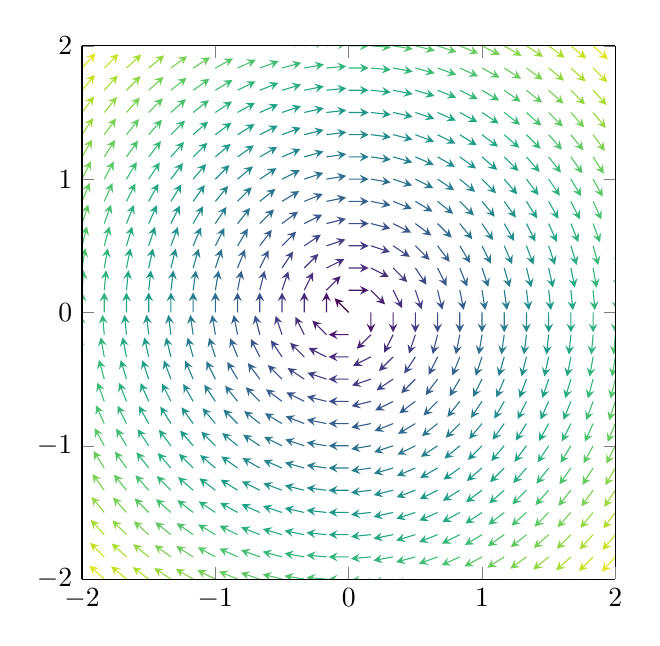
\begin{tikzpicture}
      \begin{axis}[
         xmin = -2, xmax = 2,
         ymin = -2, ymax = 2,
         zmin = 0, zmax = 1,
         axis equal image,
         xtick distance = 1,
         ytick distance = 1,
         view = {0}{90},
         scale = 1.25,
         height=7cm,
         colormap/viridis,
      ]
         \addplot3[
            point meta = {sqrt(x^2+y^2)},
            quiver = {
               u = {y/sqrt(x^2+y^2)},
               v = {-x/sqrt(x^2+y^2)},
               scale arrows = 0.15,
            },
            quiver/colored = {mapped color},
            -stealth,
            domain = -2:2,
            domain y = -2:2,
         ] {0};   
      \end{axis}
   \end{tikzpicture}
   \caption{Champs de vecteurs \( f(x, y) = (-y, x) \)}
\end{figure*}
On utilise alors un vocabulaire spécifique dans ce cadre:
\begin{itemize}
   \item On appelle \textbf{courbe intégrable} une solution maximale de l'équation.
   \item On appelle \textbf{orbite} une courbe géométrique image d'une solution de l'équation.
   \item On appelle \textbf{point stationnaire} les points tels que le champs de vecteur s'annule.
   \item On appelle \textbf{iscolines} les points tels qu'une des composantes du champs de vecteurs s'annulent.
\end{itemize}
On peut alors montrer que dans ce cadre particulier, si deux solutions maximales \( y_1, y_2 \) ont un point commun, alors elles sont \textbf{translatées} l'une de l'autre, et en conséquences, elles ont la même orbite. En outre la justification du terme d'orbite sera justifiée plus loin.
\subsection*{\subsecstyle{Flot réduit{:}}}
Dans ce cadre le flot se réduit simplement car si \( y_{t_0, y_0} \) est une solution maximale, alors la fonction translatée \( y_{0, y_0}(t + t_0)\) vérifie la même condition. En outre, quitte à translater, se ramener à l'étude des solutions maximales pour les conditions initiales \( (0, y_0) \). Par suite, le \textbf{flot réduit} de ce type d'équation s'écrit donc:
\[ 
   \begin{aligned}
      \Phi : D &\longrightarrow \K^n \\
      (t, y_0) &\longmapsto y_{0, y_0}(t)
   \end{aligned} 
\]
Si on fixe \( t \in \R \) et qu'on pose \( U_t = \left\{ y_0 \in \K^n \; ; \; t \in I_{0, y_0} \right\}  \), alors on peut voir le flot comme une application de la forme:
\[ 
   \begin{aligned}
      \Phi_t : U_t &\longrightarrow \K^n \\
      y_0 &\longmapsto \Phi(t, y_0) = y_{0, y_0}(t)
   \end{aligned}
\]
Qui s'intérprète alors réelement comme un opérateur d'évolution qui à un état \( y_0 \) au temps \( 0 \) associe l'état \( y_0(t) \) au temps \( t \). En particulier on montre les propriétés suivantes:
\[ 
   \begin{cases}
      \Phi_0 = \text{Id}\\
      \Phi_{t_2} \circ \Phi_{t_1} = \Phi_{t_1+t_2}\\
      \Phi_{t}^{-1} = \Phi_{-t}
   \end{cases} 
\]
Ceci définit en fait une \textbf{action du groupe} \( (\Phi_t)_{t \in \R}\) sur l'ensemble des 


